\subsection{Runder Stab, beidseitig eingespannt} \label{sec:auswertung_beidseitig_rund}
Es wurde eine geeignete Masse gewählt und fünfmal gewogen,
wobei sich eine mittlere Masse von \SI{1005.980 \pm 0.074}{\gram} ergab.

\begin{table}
\centering
\caption{Wiederholte Messung des benutzten Gewichts.}
% \label{tab:todo}
% \sisetup{table-format=2.1}
\begin{tabular}{c}
\toprule
$m \mathbin{/} \si{\gram}$ \\
\midrule
\num{1005.9} \\
\num{1005.9} \\
\num{1006.0} \\
\num{1006.0} \\
\num{1006.1} \\
\bottomrule
\end{tabular}
\end{table}


In \autoref{tab:durchbiegung3} sind die Durchbiegung ohne Last ($D_\text{0}$), unter Last ($D_\text{M}$) und die tatsächliche Durchbiegung ($D$) mit der Position der Messuhr ($x$) aufgelistet.

\begin{table}
\centering
\caption{Durchbiegung des runden Stabes nach $x$-Abstand.}
\label{tab:durchbiegung3}
% \sisetup{table-format=2.1}
\begin{tabular}{c c c c}
\toprule
$x \mathbin{/} \si{\centi\meter}$ &
$D_0 \mathbin{/} \si{\micro\meter}$ &
$D_\text{M} \mathbin{/} \si{\micro\meter}$ &
$D \mathbin{/} \si{\micro\meter}$ \\
\midrule
\expandableinput{build/table_beidseitig_rund.tex}
\bottomrule
\end{tabular}
\end{table}

\FloatBarrier

Für die rechte Seite ($x \leq \frac{L}{2}$) wurde $D(x)$ gegen den Linearisierungsterm $3L^2x-4x^3$ aufgetragen (siehe \autoref{fig:regression3}), für die linke gegen $4x^3-12Lx^2+9L^2x-L^3$ (siehe \autoref{fig:regression4}).
Mithilfe von NumPy kann dann jeweils eine Regressionsgerade $D(x) = k_{3,4} \cdot x + c_{3,4}$ berechnet werden.
Deren Parameter sind
\begin{align*}
  k_3 &=
  \SI[{scientific-notation = true, separate-uncertainty = true}]
    {1.1(5)e-5}{\meter\tothe{-2}} \\
  c_3 &= \SI{-0.8 \pm 0.8}{\micro\meter}
\intertext{für die rechte und}
  k_4 &=
  \SI[{scientific-notation = true, separate-uncertainty = true}]
    {3.3(10)e-5}{\meter\tothe{-2}} \\
  c_4 &= \SI{-4.6 \pm 1.9}{\micro\meter}
\end{align*}
für die linke Seite.


Das Flächenträgheitsmoment $\mathbf{I}$ wird aus \autoref{sec:auswertung_einseitig_rund} übernommen.
%
% Die Gewichtskraft $F_G = g \cdot m$ ist durch die Erdbeschleunigung und die zuvor bestimmte Masse gegeben.

Schließlich sind
\begin{align*}
  E_\text{rechts}
  &= \frac{F_G}{2 k_3 \mathbf{I}}
  % Welch unintuitive Schreibweise! :/
  = \SI[{scientific-notation = true, separate-uncertainty = true}]{4.0(20)e7}{\newton\per\square\milli\meter} \\
  E_\text{links}
  &= \frac{F_G}{2 k_4 \mathbf{I}}
  % Welch unintuitive Schreibweise! :/
  = \SI[{scientific-notation = true, separate-uncertainty = true}]{1.3(04)e7}{\newton\per\square\milli\meter} \\
  \bar{E}
  % Welch unintuitive Schreibweise! :/
  &= \SI[{scientific-notation = true, separate-uncertainty = true}]{2.6(10)e7}{\newton\per\square\milli\meter}
  \tag{arithmetisches Mittel} \\
\end{align*}
die gesuchten Elastizitätsmoduln.

% Die Messunsicherheit des Elastizitätsmoduls lässt sich gemäß der Gaußschen Fehlerfortpflanzung nach
% \begin{equation*}
%   \symup{\Delta}E = \frac{\partial E}{\partial m} \cdot \symup{\Delta}m
% \end{equation*}
% berechnen.


\begin{figure}
  \centering
  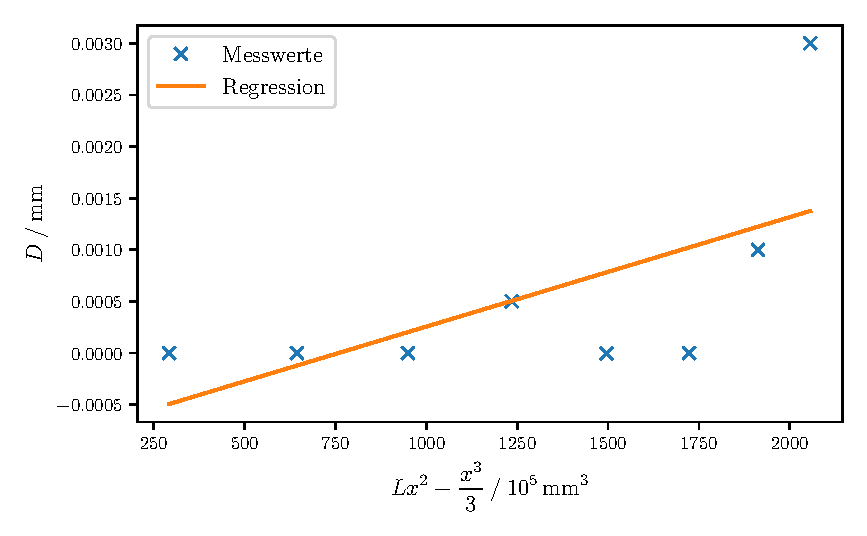
\includegraphics[scale=0.8]{build/plot_beidseitig_rund_rechts.pdf}
  \caption{Durchbiegung eines beidseitig eingespannten runden Stabes, aufgetragen gegen einen Linearisierungsterm: rechte Seite.}
  \label{fig:regression3}
\end{figure}

\begin{figure}
  \centering
  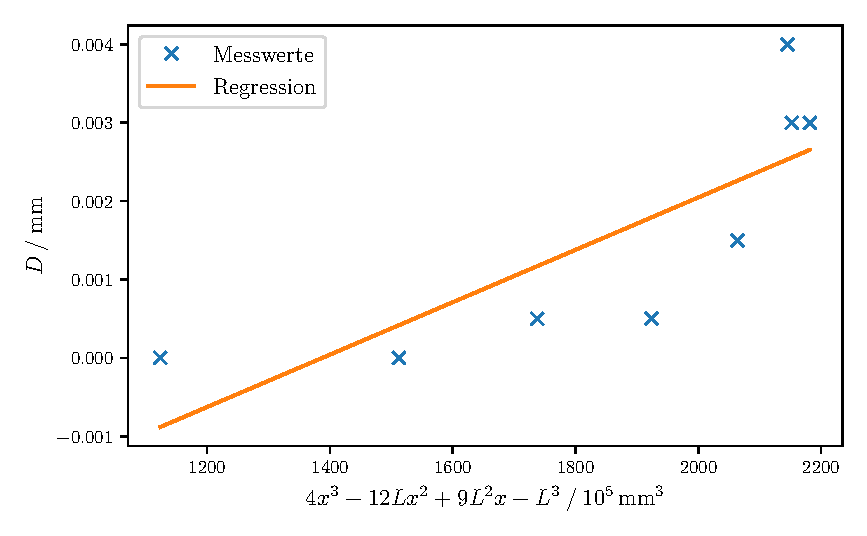
\includegraphics[scale=0.8]{build/plot_beidseitig_rund_links.pdf}
  \caption{Durchbiegung eines beidseitig eingespannten runden Stabes, aufgetragen gegen einen Linearisierungsterm: linke Seite.}
  \label{fig:regression4}
\end{figure}
